% 4-7 pages
\subsection{Key-value Databases}
\label{analysis-kv-db}
The main selling point of key-value databases is that they are quite flexible.
Lookups are very fast since all data is connected to a single, unique key. The
values can of course be of any type as well, meaning that one is not tied to a
specific schema -- anything one wants to store can be stored. Of course, this
means that the only way of querying the data is via its (primary) key. Thus, if
for any reason one would need to get the data by some other way, a key-value
database might not be the best choice.

Because of this ``constraint'', any sort of relationship becomes a hassle to
deal with in a key-value database. Since queries are done with the keys only,
connecting two items meant two queries.

The main advantage of using a key-value database for Bithoven is that the
project is quite read-heavy. The only times writes are performed is when a user
creates/deletes/modifier a playlist, and when new data is added by the
administrators. The absolute majority of the time, users would only perform read
operations -- which key-value databases can be quite performant with. However,
as we will soon discuss, this alone does not mean that it is a viable option for
our project.

For Bithoven, a key-value database does not fit well for a couple of main
reasons. The first reason is that our project is quite relationship-heavy. From
a piece (a track), we want to be able to find its composer, its performers,
album, and its performances. This is the case for many of the models, and in
some cases we want to be able to go both ways. Implementing this in a key-value
database would be quite cumbersome, since it would mean a lot of queries to get
the data we want.

\subsection{Document Databases}
\label{analysis-doc-db}

It can be quite natural to think of Bithoven in terms of documents, which is the
case for many database applications -- and one of the reasons why document
databases are so tempting. We have a lot of models, many of them in some way
connected with one another, and being able to fetch a document of this could be
very nice. However, there would be a \emph{lot} of wasted space if each document
should hold its relationships entirely. On the other hand, if the documents
contained references to its related documents, multiple queries
for---potentially---large documents would be needed to get the data the
application requires. 

Much of Bithoven's data storage has more to do with relationships than
properties. For instance, a \emph{playlist} in Bithoven is by itself nothing
more than a title. All the useful data -- i.e. who owns it, what performances it
contains -- is neither a property of the playlist nor the performance. Thus,
playlist documents would only contain a single property. Document databases are
less than ideal for relationship-heavy datasets, which makes it difficult
finding any real advantages of them for our use case.

Bithoven is a read-heavy application indeed, as briefly discussed in section
\ref{analysis-kv-db}. Scaling a document database for reading is often as simple
as adding more read slaves to the replica set. This is quite attractive for
Bithoven. However, it is questionable if it is enough of an attraction to make
document databases worth it. We still have the previously described issues to
worry about, and many other NoSQL databases scale easily enough for reads as
well.

This all leads to the fact that document databases is not the best of fit for
Bithoven, and thus the quest for the perfect NoSQL database type continues.

\subsection{Graph Databases}
\label{analysis-graph-db}

% Cons
One downside of Graph Databases is that the architecture makes it difficult to distribute the database over multiple servers. Since a node can point to any other node, relationships across servers will reduce the performance of the system. All benefits from faster graph traversal will be eliminated when server routing creates a big performance bottleneck.

% Pros
Just like relational databases, a Graph Database is consistent within a single server. Implementations like \emph{Neo4j} is fully ACID compliant. Changes are made through transactions which are either fully successful or completely rolled back. Graph Databases have great performance when traversing a graph and is useful for applications like social graphs, routing, and recommendation engines.

% Our project - benefits: advanced relationships
In our project, there are a lot of different relationships between data items that could benefit from being implemented as a Graph Database. One example is the relationship between a performer and a performance. The same performer can have multiple roles in a performance, for example being both the conductor and the soloist. With a Graph Database, this can be modeled with two relationships between two nodes, each with a different relationship type. In a relational database, this would have to be implemented with an extra table between performer and performance where the type of the relationship could be specified. Another way could also be to have multiple instances of the same performer, but each having a different performer type.

% Our project - benefits: advanced read queries are fast
The most common use cases in our project is different types of data retrieval. This includes searching with a keyword, or a specific constraint. For example, ``List all performances of any piece composed by Brahms''. This type of query would require multiple joins in a relational database system, where the Composer, Piece, and Performance tables would have to be joined and filtered. When using a Graph Database, this type of query could be done using graph traversal instead. This would provide better performance, especially once the tables become large. The relationships would also always be modeled in the database, whereas in a relational system, they would need to be recalculated for every query. Although out of scope for this project, future features that would be very reasonable for this kind of application could include even more constraints where graph traversal would deliver good performance. For example, ``List all performances of Beethovens symphonies conducted by Herbert von Karajan''.

% Our project - downsides: scalability
The biggest downside of using a Graph Database for our project is the difficulty to scale the database. Since the major benefit of a Graph Database is the performance gains of graph traversal, sharding the database and placing different nodes on different servers would most likely eliminate these performance gains. However, there is a possibility to scale the system for better read-access and availability by using multiple read-only slave servers. Our project would really take advantage of this, since most of the data in the database are not subject to frequent change. A \emph{piece} in the database will always be composed by the same composer (unless there is a music history breakthrough) and the piece will always be part of the same content group. This means that consistency would not be a major problem.

% Our project - where changes are made
The part of this project where most changes are made to the database are the changes initiated by the user. This includes creating and deleting playlists, and adding and removing performances to or from a playlist. This type of data is user specific, so quick consistency throughout the database is not a big concern. However, losing the changes would be frustrating for user. But this data loss would not result in lost sales or critical data.

% Our project - sharding the database
A Graph Database could be scaled by sharding the data based on domain-specific knowledge which could be managed in the application. This would probably become a bigger challenge as the database grows, since there are no suitable attribute in our project to divide the data by. All performances, composers, and performers in the database should be available for all users to search for, list by, or put in their playlists.

\subsection{Column Databases}
\label{analysis-col-db}

% Pros - Column-oriented
A Column-Oriented Database makes data processing faster when data from the same column needs to be processed from multiple rows. This is a typical use case in data warehouses and analytics where it is not so common to process all columns of a row at the same time.
Since compression work on localized subsets of data, data stored together by column will often require less computation to acquire a high compression rate. When the data in a column is sorted, even higher compression can be acquired by storing delta values between columns instead of absolute values.

% Cons - Column-oriented
Just as Column-Oriented Databases are advantageous when processing data from the same column, they are disadvantageous when processing data from the same row. The different columns of a row are scattered in storage, and requires retrieval from each column store to assemble the row. This can however be slightly improved by using caching and projections.

% Pros - Column-Family Store
In a Column-Family Store it is easy to add and remove columns from a single row since different rows can have different columns. In a relational database, this would require the schema to change and be harder to do.
Because every node in the cluster are equal, it is very easy to scale a Column-Family Store by simply adding more nodes. This can improve capacity, availability, and read/write performance, depending on how the system is configured.

% Cons - Column-Family Store
The Column-Family store Cassandra does not have transactions, but rather a write is only atomic at the row level. This means that rollbacks must be implemented at the application level, or by using an external transaction system like \emph{ZooKeeper}.
Column-Family stores also makes it hard to create prototypes where queries need to change frequently. When changing the queries, the design of the column family will probably have to change as well.

% Our project - Pros
The data model in this project requires tables where relationships are either optional or unspecified. For example, a performance could have one or one hundred different performers, and a performance could be part of an album and/or a content group. Implementing this in a relational database would require an extra linking table between performance and performer. All performances would need to have columns with an optional foreign key for album and content group, which would sometimes unnecessarily take up space in the database. A Column Database could implement the performance table using a column family for performers. The number of columns could vary for each row depending on how many performers a particular piece has. Other fields -- album and content group -- could be excluded from the performances which does have this, without it taking up extra space in the database.

% Our project - Cons
A downside with using a Column Database is that the columns for a row is often scattered across multiple disks and servers. In this project, it is very common to list all information about a row every time it is accessed. For example when playing a performance, the application should retrieve and display all relevant metadata, e.g. name, length, performers, composers, album, content group, etc. There are not many functions which would benefit from column data being stored contiguously in memory.

% Our project - Pros
A benefit with with using a Column Database for our project is the ease of scaling it. New nodes can easily be added to the database cluster to extend the storage capabilities, as well as availability. Since this project does not require many frequent changes to the database, it can be configured to have very fast read performance and consistent write performance.

\subsection{Our choice}
We have decided to use a Graph Database for our application. There are multiple reasons for this
choice and we will describe each in more detail. To better understand the reasons, we have
included a Graph Database data model to show how the data is related.

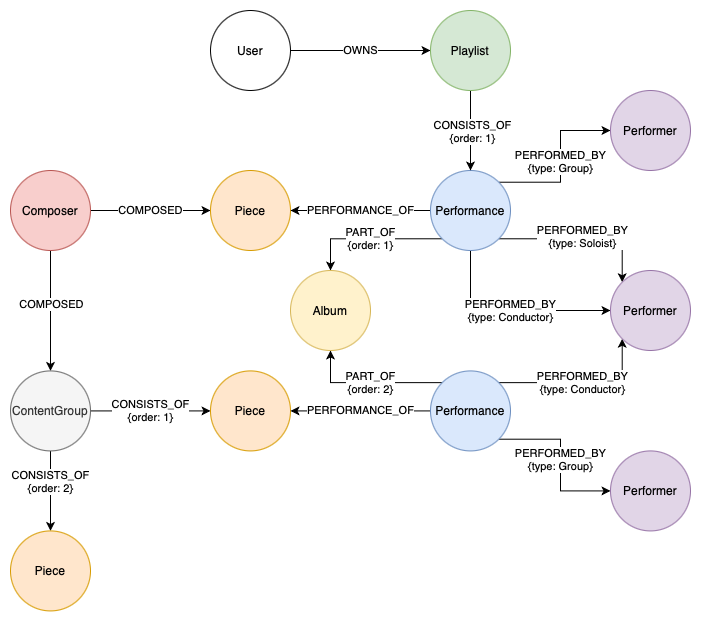
\includegraphics[scale=0.35]{graph-dm.png}

% No good main aggregate
There are no obvious main aggregate for our application. Some of the main functions of the
application is to view the data in a number of different views. A Graph Database does not have good
capabilities to store aggregate data, but can calculate an aggregate very fast. For example, one of
the functions in the application is to list all performances of a certain piece. This could be
modelled as an aggregate in all other types of NoSQL databases, but would have to be recalculated
for every query in a Graph Database, as well as a relational database. However, some other features
are to list all performances on a certain album, all performances by a certain performer, or all
performances on a certain playlist. This would require either redundant aggregates in other NoSQL
databases, or using foreign keys and create the new aggregates with application logic. Because there
are so many different aggregates with redundant data, we think that the capability to recreate the
aggregates from atomic parts in an effective way is preferable than having a few aggregates be fast
and others be slow.

% Main use cases are relationship oriented
The data for our application is naturally relationship-oriented and the relationships themselves are
just as important as the data. For example, a Composer have written Pieces, which are performed in
Performances by Performers. The data about a Piece is just as important as who wrote the piece and
which performances there are of it. This type of relationship based data fits very comfortably into
a Graph Database model. As can be seen in the attached data model, the data can easily be described
through nodes and relationships, even though the data have a semi-complicated structure. The other
NoSQL database types are more suited for aggregate or hierarchical data with a specific entry point.
For our data, almost every node can be -- and will be -- used as an entry point to find related
data. Because of this, relationships are a perfomant way to create the information needed about a
certain node. For example, a user might want to list all performances of a certain Performer. The
specific performer node can be used as an entry point in the database, and relevant data can be
traversed through the graph. The Performer node has relationships to all Performances, which have
relationships to which Piece it is a Performance of. The Piece could in turn be part of a
ContentGroup, and finally be written by a Composer. In another example, a Playlist or Album can be
used as the entry point, and provide just as performant graph traversal.

% Most of the data will be read-only, meaning scaling can be done in a controlled way
One of the big downsides of a Graph Database compared to other NoSQL databases is that it does not
scale as well. This is a downside for our application as well. However, since most of the data is
read-only the scaling can be performed in a controlled way. Read-access scaling is well supported
in Graph Databases which would be the biggest bottleneck of our application. The majority of the
data is not added or modified by the users, but rather through administrators.
Because of this, data can be added in a controlled way where the database can be migrated to
bigger hardware for vertical scaling when needed.

% Writable user data can be isolated and sharded
The data that is updated by the users -- playlists and user accounts -- will grow in an uncontrolled
way. To be able to cope with this, this data can eventually be broken out on a separate Graph
Database shard, or on another type of NoSQL database. The user data has a model more suited for the
other NoSQL types compared to the read-only data. It can use an aggregate with the user email as its
key, and user information and playlists as its value/document/columns.  Each playlist needs to hold
the key of each of its added performances to be able to access them. This is slower than a direct
relationship in a Graph Database, but key index lookups are still a fast way to retrieve data, and
the only way in most other NoSQL databases. The keys give many different entry points in the
database which each requires a key index lookup, but the performance lost is probably worth the
added scalability. However, for the scope of this project, the user data are also modelled in the
main graph database.

% Because of atomic parts, the query language can easily be used to create more advanced aggregates without changing the data in any way
In our application we want the user to be able to search for and list data in many different ways.
There could be many different criteria that the user might want to filter the data by. For example
to list all performances of any piece by a certain composer with their a specific orchestra and
conductor. This is not possible in our application right now, but can easily be added in a Graph
Database without changing the data. This is possible because Graph Databases uses atomic data
without aggregates and a query language to access the data. To support the scenario described above
only a new query would need to be created and incorporated into the application. This is very
beneficial to secure that our application is easy to continue to develop and add new features to.
